\documentclass[a4paper]{article}
% Этот шаблон документа разработан в 2014 году
% Данилом Фёдоровых (danil@fedorovykh.ru) 
% для использования в курсе 
% <<Документы и презентации в \LaTeX>>, записанном НИУ ВШЭ
% для Coursera.org: http://coursera.org/course/latex .
% Исходная версия шаблона --- 
% https://www.writelatex.com/coursera/latex/5.3

% В этом документе преамбула

\usepackage{siunitx}
%%% Работа с русским языком
%\usepackage{cmap}					% поиск в PDF
%\usepackage{mathtext} 				% русские буквы в формулах
%\usepackage[T2A]{fontenc}			% кодировка
%\usepackage[utf8]{inputenc}			% кодировка исходного текста
%\usepackage[english,russian]{babel}	% локализация и переносы
%\usepackage{indentfirst}
%\frenchspacing
%
%\renewcommand{\epsilon}{\ensuremath{\varepsilon}}
%\newcommand{\phibackup}{\ensuremath{\phi}}
%\renewcommand{\phi}{\ensuremath{\varphi}}
%\renewcommand{\varphi}{\ensuremath{\phibackup}}
%\renewcommand{\kappa}{\ensuremath{\varkappa}}
%\renewcommand{\le}{\ensuremath{\leqslant}}
%\renewcommand{\leq}{\ensuremath{\leqslant}}
%\renewcommand{\ge}{\ensuremath{\geqslant}}
%\renewcommand{\geq}{\ensuremath{\geqslant}}
%\renewcommand{\emptyset}{\varnothing}
%\renewcommand{\Im}{\operatorname{Im}}
%\renewcommand{\Re}{\operatorname{Re}}


%%% Дополнительная работа с математикой
\usepackage{amsmath,amsfonts,amssymb,amsthm,mathtools} % AMS
%\usepackage{icomma} % "Умная" запятая: $0,2$ --- число, $0, 2$ --- перечисление

%% Номера формул
%\mathtoolsset{showonlyrefs=true} % Показывать номера только у тех формул, на которые есть \eqref{} в тексте.
%\usepackage{leqno} % Нумереация формул слева

%% Свои команды
\DeclareMathOperator{\sgn}{\mathop{sgn}}
\DeclareMathOperator{\sign}{\mathop{sign}}
\DeclareMathOperator*{\res}{\mathop{res}}
\DeclareMathOperator*{\tr}{\mathop{tr}}
\DeclareMathOperator*{\rot}{\mathop{rot}}
\DeclareMathOperator*{\divop}{\mathop{div}}
\DeclareMathOperator*{\grad}{\mathop{grad}}

%% Перенос знаков в формулах (по Львовскому)
\newcommand*{\hm}[1]{#1\nobreak\discretionary{}
{\hbox{$\mathsurround=0pt #1$}}{}}

%%% Работа с картинками
\usepackage{graphicx}  % Для вставки рисунков
\graphicspath{{figures/}}  % папки с картинками
\setlength\fboxsep{3pt} % Отступ рамки \fbox{} от рисунка
\setlength\fboxrule{1pt} % Толщина линий рамки \fbox{}
\usepackage{wrapfig} % Обтекание рисунков текстом

%%% Работа с таблицами
\usepackage{array,tabularx,tabulary,booktabs} % Дополнительная работа с таблицами
\usepackage{longtable}  % Длинные таблицы
\usepackage{multirow} % Слияние строк в таблице

%%% Теоремы
\theoremstyle{plain} % Это стиль по умолчанию, его можно не переопределять.
\newtheorem{thm}{Теорема}
\newtheorem*{thm*}{Теорема}
\newtheorem{prop}{Предложение}
\newtheorem*{prop*}{Предложение}
 
\theoremstyle{definition} % "Определение"
%\newtheorem{corollary}{Следствие}[theorem]
\newtheorem{dfn}{Определение}
\newtheorem*{dfn*}{Определение}
\newtheorem{prob}{Задача}
\newtheorem*{prob*}{Задача}

 
\theoremstyle{remark} % "Примечание"
\newtheorem*{sol}{Решение}
\newtheorem*{rem}{Замечание}

%%% Программирование
\usepackage{etoolbox} % логические операторы

%%% Страница
%\usepackage{extsizes} % Возможность сделать 14-й шрифт
%\usepackage{geometry} % Простой способ задавать поля
%	\geometry{top=25mm}
%	\geometry{bottom=35mm}
%	\geometry{left=35mm}
%	\geometry{right=20mm}
 
\usepackage{fancyhdr} % Колонтитулы
%	\pagestyle{fancy}
 %	\renewcommand{\headrulewidth}{0pt}  % Толщина линейки, отчеркивающей верхний колонтитул
	%\lfoot{Нижний левый}
	%\rfoot{Нижний правый}
	%\rhead{Верхний правый}
	%\chead{Верхний в центре}
	%\lhead{Верхний левый}
	%\cfoot{Нижний в центре} % По умолчанию здесь номер страницы

\usepackage{setspace} % Интерлиньяж
%\onehalfspacing % Интерлиньяж 1.5
%\doublespacing % Интерлиньяж 2
%\singlespacing % Интерлиньяж 1

\usepackage{lastpage} % Узнать, сколько всего страниц в документе.

\usepackage{soul} % Модификаторы начертания

\usepackage{hyperref}
\usepackage[usenames,dvipsnames,svgnames,table,rgb]{xcolor}
\hypersetup{				% Гиперссылки
    unicode=true,           % русские буквы в раздела PDF
    pdftitle={Заголовок},   % Заголовок
    pdfauthor={Автор},      % Автор
    pdfsubject={Тема},      % Тема
    pdfcreator={Создатель}, % Создатель
    pdfproducer={Производитель}, % Производитель
    pdfkeywords={keyword1} {key2} {key3}, % Ключевые слова
%    colorlinks=true,       	% false: ссылки в рамках; true: цветные ссылки
    %linkcolor=red,          % внутренние ссылки
    %citecolor=black,        % на библиографию
    %filecolor=magenta,      % на файлы
    %urlcolor=cyan           % на URL
}

\usepackage{csquotes} % Еще инструменты для ссылок

%\usepackage[style=apa,maxcitenames=2,backend=biber,sorting=nty]{biblatex}

\usepackage{multicol} % Несколько колонок

\usepackage{tikz} % Работа с графикой
\usepackage{pgfplots}
\usepackage{pgfplotstable}
%\usepackage{coloremoji}
\usepackage{floatrow}
\usepackage{subcaption}
\graphicspath{{figures/}}

\renewcommand\thesubfigure{\asbuk{subfigure}}
%\addbibresource{master.bib}

\usepackage{import}
\usepackage{pdfpages}
\usepackage{transparent}
\usepackage{xcolor}
\usepackage{xifthen}

\newcommand{\incfig}[2][1]{%
    \def\svgwidth{#1\columnwidth}
    \import{./figures/}{#2.pdf_tex}
}
%\usepackage{titlesec}
%\titleformat{\section}{\normalfont\Large\bfseries}{}{0pt}{}
%----------------------STANDART:
%\titleformat{\chapter}[display]
%  {\normalfont\huge\bfseries}{\chaptertitlename\ \thechapter}{20pt}{\Huge}
%\titleformat{\section}{\normalfont\Large\bfseries}{\thesection}{1em}{}
%\titleformat{\subsection}
%  {\normalfont\large\bfseries}{\thesubsection}{1em}{}
%\titleformat{\subsubsection}
%  {\normalfont\normalsize\bfseries}{\thesubsubsection}{1em}{}
%\titleformat{\paragraph}[runin]
%  {\normalfont\normalsize\bfseries}{\theparagraph}{1em}{}
%\titleformat{\subparagraph}[runin]
%  {\normalfont\normalsize\bfseries}{\thesubparagraph}{1em}{}

\pdfsuppresswarningpagegroup=1
\pgfplotsset{compat=1.16}



%\setcounter{tocdepth}{1} % only parts,chapters,sections
%\titleformat{\subsection}{\normalfont\large\bfseries}{}{0em}{}
%\titleformat{\subsubsection}{\normalfont\normalsize\bfseries}{}{0em}{}

%\newcommand{\textover}[2]{\stackrel{\mathclap{\normalfont\mbox{#2}}}{#1}}

\author{Yaroslav Drachov\\
Moscow Institute of Physics and Technology}
%\author{Драчов Ярослав\\
%Факультет общей и прикладной физики МФТИ}
\newcommand{\veq}{\mathrel{\rotatebox{90}{$=$}}}
%\newcommand{\teto}[1]{\stackrel{\mathclap{\normalfont\tiny\mbox{#1}}}{\to}}
%\renewcommand{\thesubsection}{\arabic{subsection}}

%%\setcounter{secnumdepth}{0}

\definecolor{tabblue}{RGB}{30, 119, 180}
\definecolor{taborange}{RGB}{255, 127, 15}
\definecolor{tabgreen}{RGB}{45, 160, 43}
\definecolor{tabred}{RGB}{214, 38, 40}
\definecolor{tabpurple}{RGB}{148, 103, 189}
\definecolor{tabbrown}{RGB}{140, 86, 76}
\definecolor{tabpink}{RGB}{227, 119, 193}
\definecolor{tabgray}{RGB}{127, 127, 127}
\definecolor{tabolive}{RGB}{188, 189, 33}
\definecolor{tabcyan}{RGB}{22, 190, 207}
\pgfplotscreateplotcyclelist{colorbrewer-tab}{
{tabblue},
{taborange},
{tabgreen},
{tabred},
{tabpurple},
{tabbrown},
{tabpink},
{tabgray},
{tabolive},
{tabcyan},
}
\usepackage{csvsimple}
\usepackage{extarrows}
%\renewcommand{\labelenumii}{\asbuk{enumii})}
%\renewcommand{\labelenumiv}{\Asbuk{enumiv}}
%\newcommand{\prob}[1]{\subsubsection*{#1}}
\sisetup{output-decimal-marker = {,},separate-uncertainty = true,exponent-product = \cdot}

\usepackage{braket}
\usepackage{enumerate}
\usepackage{chngcntr}
%\counterwithin*{equation}{problem}
%\usepackage{bbold}

\newtheoremstyle{hiProb}% ⟨name ⟩ 
{3pt}% ⟨Space above ⟩1 
{3pt}% ⟨Space below ⟩1
{}% ⟨Body font ⟩
{}% ⟨Indent amount ⟩2
{\bfseries}% ⟨Theorem head font⟩
{.}% ⟨Punctuation after theorem head ⟩
{.5em}% ⟨Space after theorem head ⟩3
%{\thmname{#1} \thmnote{#3}}% ⟨Theorem head spec (can be left empty, meaning ‘normal’)⟩
{\thmnote{#3}}% ⟨Theorem head spec (can be left empty, meaning ‘normal’)⟩
\theoremstyle{hiProb} % "Определение"
%\newtheorem{hiProb}{Задача}
\newtheorem{hiProb}{}
%\usepackage{mmacells}
\newcommand{\textover}[2]{\stackrel{\mathclap{\normalfont\scriptsize\mbox{#2}}}{#1}}
\usepackage{units}
\usepackage[math]{cellspace}%
\setlength\cellspacetoplimit{2pt}
\setlength\cellspacebottomlimit{2pt}

\DeclareMathAlphabet{\mathbbold}{U}{bbold}{m}{n}

\newcommand{\normord}[1]{:\mathrel{#1}:}

\title{Домашняя работа по вычислительной математике\\
Задание 1}
\begin{document}
	\maketitle
	\section*{Тема IX. Построение общего решения}	
\begin{hiProb}[7.19]
	Найти все решения задачи на собственные значения
	\[
		\frac{y_{k+1} -2 y_k +y_{k-1}}{h^2}=(2-\lambda)
		y_k,\quad y_0=0,\quad y_N=y_{N-1},\quad
		h=\frac{1}{N}
	.\] 

\end{hiProb}
\begin{sol}
Рассмотрим эту задачу как разностное уравнение второго порядка
\[
	y_{k+1}-2y_k+ y_{k-1}=(2-\lambda)h^2 y_k
\]
или
\[
	y_{k+1}+(\lambda h^2 -4)y_k +y_{k-1}=0
.\] 
Характеристическое уравнение, соответствующее данному разностному,
есть
\[
	q^2 +(\lambda h^2 -4) q+1=0
.\] 
По теореме Виета имеем
\[
q_1= \frac{1}{q_2}
.\] 
Тогда общее решение разностного уравнения имеет вид
\[
\overline{y}_n= \alpha q_1^n +\beta q_1^{-n}
.\] 
Подстановка в левое граничное условие даёт соотношение
$\alpha+\beta=0$, тогда
\[
	\overline{y}= \alpha\left(  q_1^n-q_1^{-n} \right) 
.\] 
Теперь используем правое граничное условие
\[
	\alpha\left( q_1^N-q_1^{-N} \right) =
	\alpha\left( q_{1}^{N-1}-q_1^{-N+1} \right) 
.\] 
При $\alpha=0$ получаем тривиальное решение, которое нас не 
интересует. Тогда для того, чтобы удовлетворить этому уравнению,
должно быть выполнено \[q_1^{N}-q_1^{-N}=q_1^{N-1}-q_1^{1-N}.\]
\[
q_1^{2N}-1=q_1^{2N-1}-q_1
.\] 
\[
	(q_1^{2N-1}+1)(q_1-1)=0
.\] 
Откуда
\[
	q_1=e^{\frac{\pi(1+2k)i}{2N-1}},\
	k=0,\,1,\ldots,\,N-2;\quad
	q_1=1\text{ --- тривиальное решение}
.\] 
Подстановка полученного решения позволяет получить решение
разностного уравнения
\[
	\overline{y}_n ^{(k)}= \alpha \left( 
		\exp \left( \frac{\pi (1+2k) n i}{2N-1} \right) -
	\exp \left( - \frac{\pi (1+2k) n i}{2N-1} \right) \right) =\alpha 2 i \sin \frac{\pi(2k+1)n}{2N-1}
.\] 
Выбирая $\alpha=\frac{1}{2i}\sqrt{\frac{2}{l}} $, получаем
собственные функции
\[
	\overline{y}_n^{(k)}= \frac{2}{l}\sin \frac{\pi(2k+1)n}{2N-1}
.\] 
Подстановка собственных функций позволяет после ряда
тригонометрических преобразований найти спектр
для $k=0,\ldots,\,N-2$:
\begin{multline*}
	\lambda_{(k)}=2 - \frac{y_{m+1}^{(k)}-2 y_{m}^{(k)}+
	y_{m-1}^{(k)}}{y_m^{(k)}h^2}=\\=
	2- \frac{1}{h^2} \left( 
		\frac{\sin \frac{\pi (2k+1)(m+1)}{2N-1}  -
	2 \sin \frac{\pi (2k+1)m}{2N-1}+ \sin \frac{\pi
	(2k+1) (m-1)}{2N-1}}{\sin \frac{\pi (2k+1) m}{2N-1}}\right) =\\=2+\frac{4}{h^2} \sin^2 \frac{(2k+1)\pi}{4N-2} 
.\end{multline*} 
\end{sol}
\begin{hiProb}[7.20]
	Найти все решения задачи на собственные значения
	\[
		\frac{y_{k+1} -2 y_k +y_{k-1}}{h^2}=-\lambda
		y_k,\quad y_0=y_1,\quad y_N=y_{N-1},\quad
		h=\frac{1}{N}
	.\] 

\end{hiProb}
\begin{sol}
Рассмотрим эту задачу как разностное уравнение второго порядка
\[
	y_{k+1}-2y_k+ y_{k-1}=-\lambda h^2 y_k
\]
или
\[
	y_{k+1}+(\lambda h^2 -2)y_k +y_{k-1}=0
.\] 
Характеристическое уравнение, соответствующее данному разностному,
есть
\[
	q^2 +(\lambda h^2 -2) q+1=0
.\] 
По теореме Виета имеем
\[
q_1= \frac{1}{q_2}
.\] 
Тогда общее решение разностного уравнения имеет вид
\[
\overline{y}_n= \alpha q_1^n +\beta q_1^{-n}
.\] 
Подстановка в граничные условия даёт
\[
\left\{
\begin{aligned}
	\alpha+\beta=&\alpha q_1+ \beta q^{-1}\\
	\alpha q_1^{N-1}+\beta q_1^{1-N}=& \alpha q_1^N+\beta q_1^{-N}\\
\end{aligned}
\right.
.\] 
Откуда
\[
	\alpha \left( q_1^N-q_1^{N-1} \right) =
	\beta\left( q_1^{1-N}-q_1^{-N} \right) 
.\] 
\[
	\beta= \frac{q_1^N \left(1-q_1^{-1}\right)}{
	q_{1}^{-N}\left( q_1-1 \right) }\alpha=
	\alpha q_1^{2N-1}
.\] 
\[
	\alpha\left( 1+q_1^{2N-1} \right) =
	\alpha\left( q_1+q_1^{2N-2} \right) 
.\] 
\[
	\alpha\left( 1+ q_1^{2N-1} \right) =\alpha
	\left( q_1+q_1 ^{2N-2} \right) 
.\] 
\[
1-q_1+q_1^{2N-1}- q_1^{2N-2}=0
.\] 
\[
	\left( 1-q_1 \right) \left( 1-q_1^{2N-2} \right) =0
.\]
Следовательно
\[
	q_1^{(k)} =e^{\frac{2\pi ki}{2N-2}},\
	k=0,\,1,\ldots,\,N-2;\quad
	q_1=1\text{ --- тривиальное решение}
.\] 
Подстановка полученного решения позволяет получить решение
разностного уравнения
\[
	\overline{y}_n ^{(k)}= \alpha \left( 
		\exp \left( \frac{\pi  ki}{N-1}n \right) +
	\exp \left( \frac{\pi k i}{N-1}(2N-1-n) \right) \right) 
.\] 
\[
	\overline{y}_n ^{(k)}= \alpha \left( 
		\exp \left( \frac{\pi  ki}{N-1}n \right) +
	\exp \left( \frac{\pi k i}{N-1}(1-n) \right) \right) 
.\]
\[
	\lambda_k= \frac{1}{h^2} \left( 2-q_1 ^{(k)}- \frac{1}{q_1^{(k)}} \right) =\frac{1}{h^2}\left(  2- e^{\frac{\pi k i}{N-1}}-e^{- \frac{\pi k i }{N-1}} \right) = \frac{4}{h^2} \sin^2 \frac{\pi k}{2N-2}
.\] 
\end{sol}
\begin{hiProb}[7.10]
Найти все значения параметра $\alpha$, при котором все
решения разностного уравнения
\[
	13y_{k+1}+(13+\alpha)y_k +(\alpha+7) y_{k-1}+
	\left( \alpha+7 \right) y_{k-2}+(\alpha+1) y_{k-3}+y_{k-4}=0
\] 
будут ограничены при $k\to \infty$.
\end{hiProb}
\begin{sol}
Характеристический многочлен для разностного уравнения в данном случае есть 
\[
	g(q)=13q^5+(13+\alpha)q^4+(\alpha+7)q^3+
	(\alpha+7)q^2+\left( \alpha+1 \right) q+1=0
.\] 
Для ограниченности решения при $k\to \infty$ необходимо и
достаточно, чтобы корни уравнения  были по модулю меньшее или 
равны единице, а на границе единичного круга не было кратных
корней. Преобразуем характеристический многочлен:
\[
	g(q)=(q+1)\left(\alpha  q^3+13 q^4+7 q^2+\alpha  q+1  \right) 
.\] 
Один из корней по модулю равен единице. Теперь применим
теорему Шура-Кона для определения действительных значений
параметра $\alpha$, при которых полином
$f(q)=13 q^4+\alpha  q^3+7 q^2+\alpha  q+1 $ будет
иметь все корни внутри единичного круга. Первое из условий
теоремы выполнено: $13>1$. Найдём $f_1(z)$:
\[
	f_1(z)= 12 \left(\alpha +\alpha  z^2+14 z^3+7 z\right)
.\] 
Для $f_1(z)$ первое условие теоремы накладывает на исследуемый параметр условие $14>|\alpha|$. Далее
 \[
	 f_2(z)= -144 \left(\alpha ^2+\left(\alpha ^2-196\right) z^2-7 \alpha  z-98\right)
,\] 
откуда $196-\alpha^2>98-\alpha^2$ --- всегда верно.
\[
f_3(z)=-2032128 \left(2 \left(\alpha ^2-147\right) z-7 \alpha \right) \text{ и } \left| 2(\alpha^2-147) \right| >|7\alpha|
.\] 
Последнее неравенство верно при
\[
|\alpha|<\frac{21}{2} \text{ или } |\alpha|>14
.\] 
Собирая полученные условия на $\alpha$ получаем
\[
|\alpha|<\frac{21}{2}
.\] 
%На границах получившегося интервала лежат значения параметра,
%при которых полином $f(z)$ будет обладать корнями с модулями,
%равными 1:
%\begin{itemize}
%	\item $\alpha=-14\implies f(q)=\frac{1}{2}(q-1)\left( 26 q^3+5 q^2+19 q-2\right) $ обладает корнем $q=1$,
% \item $\alpha=$
%\end{itemize}
\end{sol}
\begin{hiProb}[7.12-2]
	Найти общее решение системы разностных уравнений (однородных и неоднородных):
	\[
	\left\{
	\begin{aligned}
		x_{n+1}&=x_n-y_n+n,\\
		y_{n+1}&= -2x_n+2n \\
	\end{aligned}
	\right.
	.\] 
\end{hiProb}
\begin{sol}
Рассмотрим однородную систему разностных уравнений
\[
\left\{
\begin{aligned}
x_{n+1}&= x_n -y_{n}, \\
y_{n+1}&=-2x_n  \\
\end{aligned}
\right.
.\] 
Для неё характеристическое уравнение будет иметь вид
\[
	\begin{vmatrix} 1-q & -1 \\ -2 & -q \end{vmatrix} =
q^2-q-2=0
.\] 
Корни данного уравнения
\[
q_1=-1,\quad q_2=2
\]
--- действительны и различны, тогда общее решение однородной
системы представляется в виде
\[
	\begin{pmatrix} x_{n} \\ y_{n} \end{pmatrix} =
	c_1 \begin{pmatrix} 1\\2 \end{pmatrix} (-1)^n+
	c_2 \begin{pmatrix} -1\\1 \end{pmatrix} 2^n
.\] 
Частное решение неоднородного уравнения будем искать в
виде
\[
\begin{pmatrix} x_n \\y_{n} \end{pmatrix} =\begin{pmatrix}a\\b  \end{pmatrix} n+ \begin{pmatrix} c\\d \end{pmatrix} 
.\] 
Подставляя в уравнение, получаем
\[
\left\{
\begin{aligned}
	a(n+1)+c&= an+c-bn-d+n \\
	b(n+1)+d&= -2an-2c+2n \\
\end{aligned}
\right.
\Leftrightarrow
\left\{
\begin{aligned}
a+bn+d&= n \\
2an+bn+b+2c+d&= 2n \\
\end{aligned}
\right.
\] 
Положим $b=1$, тогда $a=-d$ и
 \[
2an+1+2c-a=n
.\] 
Полагая $a=1 /2$ получаем $c=- 1 /4$. Откуда частное решение
неоднородной системы
 \[
\begin{pmatrix} x_{n} \\ y_{n} \end{pmatrix} =
\begin{pmatrix} 1 /2 \\ 1 \end{pmatrix} n -\begin{pmatrix}  1 /4 \\ 1/2 \end{pmatrix} 
.\] 
Общее решение исследуемой неоднородной разностной системы уравнений
представляется как сумма её частного решения и общего решения, соответствующей ей,
однородной разностной системы:
\[
\begin{pmatrix} x_n\\y_n \end{pmatrix} =
c_1\begin{pmatrix} 1\\2 \end{pmatrix} (-1)^n+ c_2 \begin{pmatrix} 
-1\\ 1\end{pmatrix} 2^n+ \begin{pmatrix} 1/2 \\ 1 \end{pmatrix} n - \begin{pmatrix} 1 / 4\\1 /2 \end{pmatrix} 
.\] 
\end{sol}
\begin{hiProb}[7.15-2]
Найти общее решение неоднородной системы разностных
уравнений
\[
\left\{
\begin{aligned}
x_{n+1}&= -2x_n +3y_n+5\cdot 2^n-6 \\
y_{n+1}&= -3x_n+8y_n +30 \cdot 2^n-2 \\
\end{aligned}
\right.
.\] 
\end{hiProb}
\begin{sol}
Сперва найдём решение однородной системы аналогично
предыдущей задаче
\[
\begin{pmatrix} x_n \\y_n \end{pmatrix} =
c_1\begin{pmatrix}1\\3  \end{pmatrix} 7^n+ c_2
\begin{pmatrix} 3\\1 \end{pmatrix} (-1)^n
.\] 
Частное решение будем искать в виде
\[
\begin{pmatrix} x_n \\ y_n \end{pmatrix} = \begin{pmatrix} a\\b \end{pmatrix} 2^n+ \begin{pmatrix} c \\d \end{pmatrix} 
.\] 
Подставляя, получаем
\[
\left\{
\begin{aligned}
	a \cdot2^{n+1}+c&=-2a\cdot 2^{n}-2c+3b\cdot 2^n+3d+
	5\cdot 2^n-6\\
	b\cdot 2^{n+1}+d &= -3a\cdot 2^n-3c+8b\cdot 2^n+8d+
	30\cdot 2^n-2\\
\end{aligned}
\right.
.\] 
Откуда
\[
\left\{
\begin{aligned}
2a&= -2a+3b+5 \\
2b&= -3a+8b+30 \\
c&= -2c+3d-6 \\
d&= -3c+8d-2 \\
\end{aligned}
\right. 
\Leftrightarrow 
\left\{
\begin{aligned}
a&= -4 \\
b&= -7 \\
c&= -3 \\
d&= -1 \\
\end{aligned}
\right.
.\] 
Следовательно, общее решение исследуемой
неоднородной системы будет иметь вид
\[
\begin{pmatrix} x_n\\y_n \end{pmatrix} =
c_1 \begin{pmatrix} 1\\3 \end{pmatrix} 7^n+c_2
\begin{pmatrix} 3\\1 \end{pmatrix} (-1)^n-
\begin{pmatrix} 4\\7 \end{pmatrix} 2^n-\begin{pmatrix} 3\\1 \end{pmatrix} 
.\] 
\end{sol}
%\begin{hiProb}[7.1]
%Найти общее решение уравнения
%\[
%2 y_n-y_{n+1}=5^n
%.\] 
%\end{hiProb}
%\begin{sol}
%Для однородной части данного уравнения составим характеристическое:
%\[
%2-q=0\implies q=2 
%.\] 
%Решение неоднородного уравнения будем искать в виде $a\cdot 5^n$:
%\[
%2a-5a=1\implies a=- \frac{1}{3}
%.\] 
%Следовательно, общим решением будет
%\[
%y_n=2^n-\frac{1}{3}\cdot 5^n
%.\] 
%\end{sol}
\section*{Тема X. Жёсткие системы ОДУ}
\begin{hiProb}[7.1]
Уравнение Ван-дер-Поля записано в виде системы второго 
порядка 
\[
	\left\{
	\begin{aligned}
		y_1'&=1000 \left( y_1- \frac{y_1^3}{3} \right) +y_2
, \\
	y_2'&=-y_1
	\end{aligned}
	\right.
.\] 
Определить тип особой точки системы. Найти, в какой
части фазового пространства задача является жёсткой.
Определить показатель жёсткости системы.
\end{hiProb}
\begin{sol}
В окрестности нуля:
	\[
	\left\{
	\begin{aligned}
	y_1'&= 1000y_1+y_2 \\
	y_2'&=-y_1
	\end{aligned}
	\right.
	.\] 
	Собственными значениями матрицы
	\[
		\begin{pmatrix} 1000 &1\\ -1 &0 \end{pmatrix} 
	\] 
будут
\[
\lambda_{1,2}= 500 \pm \sqrt{500^2-1} 
.\] 
Собственные значения положительны и различны, следовательно
особая точка данной системы --- неустойчивый узел.

Матрица Якоби данной системы:
\[
	\mathbf{J}= \begin{pmatrix}1000\left(1-y_1^2\right) & 1\\ -1&0  \end{pmatrix} 
.\] 
Её спектр:
\[
	\lambda_{1,2}=500(1-y_1^2)\pm \sqrt{500^2(1-y_1^2)^2-1} 
.\] 
Сделаем замену
\[
	x=500(1-y_1^2) \in (-\infty,\,500)
.\] 
Тогда
\[
\lambda_{1,2}=x\pm \sqrt{x^2-1} 
.\] 
При $|x|\ge 1$ получаем чисто действительные собственные значения,
при $|x|<1$ 
\[
\lambda_{1,2}=x\pm i \sqrt{1-x^2} 
\] 
--- комплексно-сопряжённые собственные значения, лежащие на единичной
окружности на комплексной плоскости. То есть при $|x|\le 1$
в полученном наборе собственных значений присутствует лишь
мягкий спектр, и, как следствие, система --- не жёсткая.
%Заметим, что
%\[
%\Re \lambda_{1,2}= \begin{cases}
%	500(1-y_1^2),& \sqrt{\frac{499}{500}} \le |y_1|\le  \sqrt{\frac{501}{500}},\\
%	500(1-y_1^2)\pm\sqrt{500^2(1-y_1^2)^2-1},&\text{иначе.}
%\end{cases}
%\]
%\[
%\Im \lambda_{1,2}= \begin{cases}
%	\pm\sqrt{1-500^2(1-y_1^2)^2},& \sqrt{\frac{499}{500}} \le |y_1|\le  \sqrt{\frac{501}{500}},\\
%	0,&\text{иначе.}
%\end{cases}
%\]

Критерием жёсткости системы для данной задачи будет наличие такихнаименьших
 положительных $\lambda$ и $\Lambda$, что
\[
|\lambda_1|\le \lambda,\quad \Re \lambda_2\le -\Lambda,\quad
|\Im \lambda_2|\le \Lambda,\quad \frac{\Lambda}{\lambda}\ll 1
.\] 
Для случая чисто действительных собственных значений последнее
неравенство автоматически выполнено, второе неравенство
накладывает обязательное условие наличия хотя бы одного
отрицательного собственного значения.
Так как для $|x|\ge 1$ выполняется неравенство
\[
|x|\ge \sqrt{x^2-1} 
,\] 
то выражение
\[
x\pm \sqrt{x^2-1} 
\] 
имеет шансы быть отрицательным лишь при отрицательных $x$.
Ну а для $x\le -1$ можно уже однозначно сказать, что
\[
\left| x+\sqrt{x^2-1} \right|\le  \left| x-\sqrt{x^2-1}  \right| 
.\] 
Согласно данному выше определению можем найти $\lambda$ и
$\Lambda$ для рассматриваемого случая:
\[
\Re \lambda_+=x-\sqrt{x^2-1} = -\Lambda
,\] 
\[
|\lambda_-|=-x-\sqrt{x^2-1} = \lambda
.\] 
Тогда критерием жёсткости системы будет оценка
\[
\frac{\Lambda}{\lambda}=\frac{x-\sqrt{x^2-1} }{x+\sqrt{x^2-1} }=2 x \left(x-\sqrt{x^2-1}\right)-1 \gg 1
.\] 
Она будет выполняться тем лучше, чем $x$ ближе к $-\infty$.
Раскладываясь по Тейлору в окрестности $-\infty$, упрощаем
оценку
\[
2 x \left(x-\sqrt{x^2-1}\right)-1 \sim 4x^2 \gg 1
.\] 
Для численной оценки выберем произвольно минимальный коэффициент жёсткости $\alpha \gg 1$ жёсткой системы. Тогда любая
система будет жёсткой, если её коэффициент жёсткости не меньше
$\alpha$. То есть
\[
4x^2 \ge \alpha
.\] 
Возвращаясь к исходным переменным, получаем условие на жёсткость системы:
\[
10^6 \left(1-y_1^2\right)^2\geq \alpha
.\] 
Вид решения зависит от параметра $\alpha$ и представлен на рис.~\ref{fig:1}.
\begin{figure}[htpb]
	\centering
	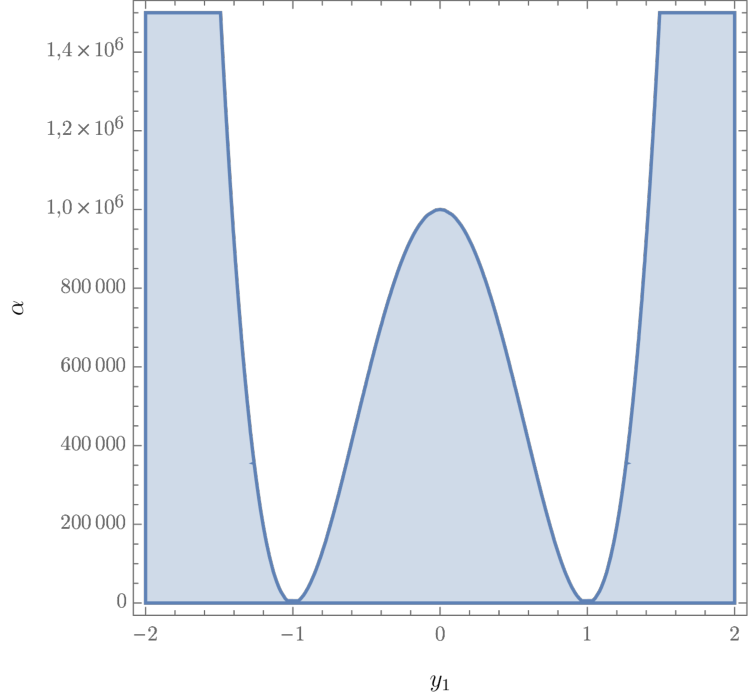
\includegraphics[width=0.8\textwidth]{1}
	\caption{}
	\label{fig:1}
\end{figure}
От $y_2$, как мы выяснили, жёсткость системы не зависит.
%Для случая комплексно-сопряжённых корней
%выбор $\lambda$ не ограничен сверху, следовательно
%при $1<x\le 1$ коэффициент жёсткости
%так же можно выбрать равным нулю.
%
%Всё это как-то странно получается\ldots
%И тогда условие жёсткости системы запишется как
%\[
%\frac{\Lambda}{\lambda}\le \frac{x+\sqrt{x^2-1} }{x-\sqrt{x^2-1} }\ll 1
%.\] 
%\[
%\frac{x-\sqrt{x^2-1} }{x+\sqrt{x^2-1} }=2 x \left(x-\sqrt{x^2-1}\right)-1\ll 1
%.\] 
%Полученная для оценки функция --- положительная и строго-убывающая на промежутке
%$\left( -\infty,\,-1 \right] $ и в точке $x=-1$ равна единице,
%следовательно необходимое условие жёсткости
%Видно, что это условие тем лучше выполнено, чем ближе
%$x$ к -1. Раскладываясь по Тейлору в данной окрестности,
%получим
%или для переменной $y_1$:
%\[
%1000 \left(1-y_1^2\right) \left(-500 \left(y_1^2-1\right)-\sqrt{500^2
%   \left(y_1^2-1\right){}^2-1}\right)-1\ll 1
%.\] 
%\[
%x\pm \sqrt{x^2-1} \le 0 \implies x \le  \mp \sqrt{x^2-1} 
%.\] 
%Задача распадается на два случая:
%\begin{enumerate}
%\item Пусть
%\[
%	\lambda_1=500(1-y_1^2)+ \sqrt{500^2(1-y_1^2)^2-1} 
%,\]
%\[
%	\lambda_2=500(1-y_1^2)- \sqrt{500^2(1-y_1^2)^2-1} 
%.\]
%\end{enumerate}
\end{sol}
\begin{hiProb}[7.2]
Получить функции устойчивости всех явных методов Рунге–Кутты с порядком аппроксимации с первого до седьмого с минимальным числом стадий.
\end{hiProb}
\begin{sol}
Так как
\[
u_{n+1}=e^{\lambda h} u_n,\quad y_{n+1}=
R(\lambda h) y_n,\quad |u_{n+1}-y_{n+1}|=O\left(h^{p+1}\right)=
O\left(z^{p+1}\right)
,\] 
где $\lambda h=z$, то у $R(z)$ и $e^z$ ряды Тейлора
совпадают вплоть до порядка аппроксимации $p$.
Известно, что для $p\le 4$ существуют ЯМРК
с числом стадий $s=p$.

Для $p$ от 1 до 4 найдутся  $s$-стадийные методы
с числом стадий равным порядку аппроксимации,
значит для таких методов функция устойчивости
$R(z)$ не будет зависеть от конкретного вида
таблицы Бутчера и будет равна
\[
	R (z)=1+z+\ldots+\frac{z^s}{s!},
\] 
Далее, после так называемого первого барьера Бутчера,
методы с $p\ge 5$ будут, как минимум $s+1$-стадийные:
\[
	p=5:\quad R(z)=1+z+ \frac{z^5}{5!}+ C_6 z^6,
\] 
\[
	p=6:\quad R(z)=1+z+\ldots+\frac{z^6}{6!}+
	C_7 z^7
,\] 
где $C_6$ и $C_7$ зависят от таблицы Бутчера.
После второго барьера Бутчера ($p\ge 7$) методы
будут как минимум $s+2$-стадийные:
\[
p=7:\quad	R(z)=1+z+\ldots+\ldots+\frac{z^7}{z!}+
	C_8 z^8 +C_9 z^9
,\]
где, как и раньше, $C_8$ и $C_9$ зависят от конкретного
вида таблицы Бутчера.
\end{sol}
\begin{hiProb}[7.3]
Вывести условия порядка для всех двухстадийных НМРК вплоть до четвертого.
\end{hiProb}
\begin{sol}
Задача решалась при помощи пакета Mathematica:

\begin{mmaCell}[moredefined={s, F, list1, list2, set},morepattern={h_, i_, j_, \#},morefunctionlocal={i, h, j, m, p}]{Input}
  s=2;
  F[h_,i_]:=f[\mmaSub{x}{n}+\mmaSub{c}{\mmaPat{i}}\mmaPat{h},\mmaSub{y}{n}+\mmaPat{h} \mmaUnderOver{\(\pmb{\sum}\)}{j=1}{s}\mmaSub{a}{\mmaPat{i},j}\mmaSub{k}{j}[\mmaPat{h}]]
  list1=CoefficientList[Normal[Series[
  \mmaSub{y}{n}+h \mmaUnderOver{\(\pmb{\sum}\)}{i=1}{s}\mmaSub{b}{i}f[\mmaSub{x}{n}+\mmaSub{c}{i}h,\mmaSub{y}{n}+h\mmaUnderOver{\(\pmb{\sum}\)}{j=1}{s}\mmaSub{a}{i,j}\mmaSub{k}{j}[h]],\{h,0,4\}]]//.\{
  Derivative[i_][\mmaSub{k}{j_}][_] \(\pmb{\to}\)Derivative[\mmaUnd{i},0][F][0,\mmaUnd{j}],
  \mmaSub{k}{i_}[0]\(\pmb{\to}\)f[\mmaSub{x}{n},\mmaSub{y}{n}]\},\mmaUnd{h}];
  list2=CoefficientList[Normal[Series[
  u[\mmaSub{x}{n}+h],\{h,0,4\}]]
  //.Derivative[i_][u][_] \(\pmb{\to}\)  
  D[f[\mmaSub{x}{n},u[\mmaSub{x}{n}]],\{\mmaSub{x}{n},\mmaUnd{i}-1\}]/.u[\mmaSub{x}{n}]\(\pmb{\to}\)\mmaSub{u}{n},\mmaUnd{h}];
  set=Table[Derivative[m,p][f][\mmaSub{x}{n},\mmaSub{u}{n}],
  \{m,0,3\},\{p,0,3-m\}]//Flatten;
  Map[#==0&,DeleteCases[CoefficientList[
  #,set]&/@Flatten[\{list1-list2//Thread\}/.\mmaSub{y}{n}\(\pmb{\to}\)\mmaSub{u}{n}
  ],0,\mmaDef{\(\pmb{\infty}\)}]//Flatten]//Simplify
\end{mmaCell}

\begin{mmaCell}[addtoindex=5]{Output}
  \{\mmaSub{b}{1}+\mmaSub{b}{2}==1,2 \mmaSub{b}{1} \mmaSub{c}{1}+2 \mmaSub{b}{2} \mmaSub{c}{2}==1,2 \mmaSub{b}{1} (\mmaSub{a}{1,1}+\mmaSub{a}{1,2})+2
\mmaSub{b}{2} (\mmaSub{a}{2,1}+\mmaSub{a}{2,2})==1,3 \mmaSub{b}{1} \mmaSubSup{c}{1}{2}+3 \mmaSub{b}{2} \mmaSubSup{c}{2}{2}==1,6 \mmaSub{b}{1} (\mmaSub{c}{1}
\mmaSub{a}{1,1}+\mmaSub{c}{2} \mmaSub{a}{1,2})+6 \mmaSub{b}{2} (\mmaSub{c}{1} \mmaSub{a}{2,1}+\mmaSub{c}{2} \mmaSub{a}{2,2})==1,3 \mmaSub{b}{1} \mmaSub{c}{1}
(\mmaSub{a}{1,1}+\mmaSub{a}{1,2})+3 \mmaSub{b}{2} \mmaSub{c}{2} (\mmaSub{a}{2,1}+\mmaSub{a}{2,2})==1,6 \mmaSub{b}{1} (\mmaSubSup{a}{1,1}{2}+\mmaSub{a}{1,1}
\mmaSub{a}{1,2}+\mmaSub{a}{1,2} (\mmaSub{a}{2,1}+\mmaSub{a}{2,2}))+6 \mmaSub{b}{2} (\mmaSub{a}{1,1} \mmaSub{a}{2,1}+\mmaSub{a}{1,2} \mmaSub{a}{2,1}+\mmaSub{a}{2,2}
(\mmaSub{a}{2,1}+\mmaSub{a}{2,2}))==1,3 \mmaSub{b}{1} \mmaSup{(\mmaSub{a}{1,1}+\mmaSub{a}{1,2})}{2}+3 \mmaSub{b}{2} \mmaSup{(\mmaSub{a}{2,1}+\mmaSub{a}{2,2})}{2}==1,4
\mmaSub{b}{1} \mmaSubSup{c}{1}{3}+4 \mmaSub{b}{2} \mmaSubSup{c}{2}{3}==1,8 \mmaSub{b}{1} \mmaSub{c}{1} (\mmaSub{c}{1} \mmaSub{a}{1,1}+\mmaSub{c}{2}
\mmaSub{a}{1,2})+8 \mmaSub{b}{2} \mmaSub{c}{2} (\mmaSub{c}{1} \mmaSub{a}{2,1}+\mmaSub{c}{2} \mmaSub{a}{2,2})==1,12 (\mmaSub{b}{1} (\mmaSubSup{c}{1}{2}
\mmaSub{a}{1,1}+\mmaSubSup{c}{2}{2} \mmaSub{a}{1,2})+\mmaSub{b}{2} (\mmaSubSup{c}{1}{2} \mmaSub{a}{2,1}+\mmaSubSup{c}{2}{2} \mmaSub{a}{2,2}))==1,\mmaSub{b}{1}
(\mmaSub{c}{1} (\mmaSubSup{a}{1,1}{2}+\mmaSub{a}{1,2} \mmaSub{a}{2,1})+\mmaSub{c}{2} \mmaSub{a}{1,2} (\mmaSub{a}{1,1}+\mmaSub{a}{2,2}))+\mmaSub{b}{2}
(\mmaSub{c}{1} \mmaSub{a}{2,1} (\mmaSub{a}{1,1}+\mmaSub{a}{2,2})+\mmaSub{c}{2} (\mmaSub{a}{1,2} \mmaSub{a}{2,1}+\mmaSubSup{a}{2,2}{2}))==\mmaFrac{1}{24},4
\mmaSub{b}{1} \mmaSubSup{c}{1}{2} (\mmaSub{a}{1,1}+\mmaSub{a}{1,2})+4 \mmaSub{b}{2} \mmaSubSup{c}{2}{2} (\mmaSub{a}{2,1}+\mmaSub{a}{2,2})==1,8 \mmaSub{b}{1}
(\mmaSub{a}{1,1}+\mmaSub{a}{1,2}) (\mmaSub{c}{1} \mmaSub{a}{1,1}+\mmaSub{c}{2} \mmaSub{a}{1,2})+8 \mmaSub{b}{2} (\mmaSub{a}{2,1}+\mmaSub{a}{2,2})
(\mmaSub{c}{1} \mmaSub{a}{2,1}+\mmaSub{c}{2} \mmaSub{a}{2,2})==1,\mmaSub{b}{1} (\mmaSub{c}{2} \mmaSub{a}{1,2} (\mmaSub{a}{2,1}+\mmaSub{a}{2,2})+\mmaSub{c}{1}
(2 \mmaSubSup{a}{1,1}{2}+2 \mmaSub{a}{1,1} \mmaSub{a}{1,2}+\mmaSub{a}{1,2} (\mmaSub{a}{2,1}+\mmaSub{a}{2,2})))+\mmaSub{b}{2} (\mmaSub{c}{1} (\mmaSub{a}{1,1}+\mmaSub{a}{1,2})
\mmaSub{a}{2,1}+\mmaSub{c}{2} (\mmaSub{a}{1,1} \mmaSub{a}{2,1}+\mmaSub{a}{1,2} \mmaSub{a}{2,1}+2 \mmaSub{a}{2,2} (\mmaSub{a}{2,1}+\mmaSub{a}{2,2})))==\mmaFrac{5}{24},\mmaSub{b}{2}
(\mmaSubSup{a}{1,1}{2} \mmaSub{a}{2,1}+\mmaSub{a}{1,1} \mmaSub{a}{2,1} (\mmaSub{a}{1,2}+\mmaSub{a}{2,2})+\mmaSubSup{a}{2,2}{2} (\mmaSub{a}{2,1}+\mmaSub{a}{2,2})+\mmaSub{a}{1,2}
\mmaSub{a}{2,1} (\mmaSub{a}{2,1}+2 \mmaSub{a}{2,2}))+\mmaSub{b}{1} (\mmaSubSup{a}{1,1}{3}+\mmaSubSup{a}{1,1}{2} \mmaSub{a}{1,2}+\mmaSub{a}{1,1} \mmaSub{a}{1,2}
(2 \mmaSub{a}{2,1}+\mmaSub{a}{2,2})+\mmaSub{a}{1,2} (\mmaSub{a}{1,2} \mmaSub{a}{2,1}+\mmaSub{a}{2,2} (\mmaSub{a}{2,1}+\mmaSub{a}{2,2})))==\mmaFrac{1}{24},4
\mmaSub{b}{1} \mmaSub{c}{1} \mmaSup{(\mmaSub{a}{1,1}+\mmaSub{a}{1,2})}{2}+4 \mmaSub{b}{2} \mmaSub{c}{2} \mmaSup{(\mmaSub{a}{2,1}+\mmaSub{a}{2,2})}{2}==1,3
\mmaSub{b}{2} (\mmaSubSup{a}{1,1}{2} \mmaSub{a}{2,1}+\mmaSubSup{a}{1,2}{2} \mmaSub{a}{2,1}+2 \mmaSub{a}{1,2} \mmaSub{a}{2,1} (\mmaSub{a}{2,1}+\mmaSub{a}{2,2})+3
\mmaSub{a}{2,2} \mmaSup{(\mmaSub{a}{2,1}+\mmaSub{a}{2,2})}{2}+2 \mmaSub{a}{1,1} \mmaSub{a}{2,1} (\mmaSub{a}{1,2}+\mmaSub{a}{2,1}+\mmaSub{a}{2,2}))+3
\mmaSub{b}{1} (3 \mmaSubSup{a}{1,1}{3}+6 \mmaSubSup{a}{1,1}{2} \mmaSub{a}{1,2}+\mmaSub{a}{1,2} (\mmaSub{a}{2,1}+\mmaSub{a}{2,2}) (2 \mmaSub{a}{1,2}+\mmaSub{a}{2,1}+\mmaSub{a}{2,2})+\mmaSub{a}{1,1}
\mmaSub{a}{1,2} (3 \mmaSub{a}{1,2}+2 (\mmaSub{a}{2,1}+\mmaSub{a}{2,2})))==1,4 \mmaSub{b}{1} \mmaSup{(\mmaSub{a}{1,1}+\mmaSub{a}{1,2})}{3}+4 \mmaSub{b}{2}
\mmaSup{(\mmaSub{a}{2,1}+\mmaSub{a}{2,2})}{3}==1\}
\end{mmaCell}
\end{sol}
\end{document}
